\documentclass[12pt]{article}
\usepackage{authblk}
\usepackage[english]{babel}
% or whatever
\usepackage[utf8]{inputenc}
\usepackage{times}
\usepackage{amssymb}
\usepackage{amsmath}
\usepackage{amsthm}
\usepackage{float}
\usepackage{graphicx}
\usepackage{subcaption}
\usepackage{floatflt}
\usepackage{dsfont}	
%\usepackage{subscript}
\usepackage{enumitem}
\usepackage{amsbsy}
\usepackage{fixmath}
\usepackage{mathtools}
\usepackage{breqn}
\usepackage{booktabs}
\usepackage{hyperref}
\usepackage[english]{cleveref}
\usepackage{tabularx}
\usepackage{xcolor}
\usepackage{breqn}
\usepackage{fullpage}
\usepackage{tikz}

\usepackage{verbatim}

\usepackage{algorithm}
\usepackage[noend]{algpseudocode}

\parindent0pt

\hypersetup{
	colorlinks,
	citecolor=orange,
	filecolor=indigo,
	linkcolor=orange,
	urlcolor=blue
}


\DeclareMathOperator*{\argmin}{arg min}
\DeclareMathOperator*{\ds}{ds}

\begin{document}
	\author{Marcel A. Brusius,
			Leif Eric Goebel}
	\date{\today}
	\title{Results Exercise 2}
	\maketitle
	\begin{tikzpicture}[remember picture,overlay]
	\node [anchor=north west, inner xsep=0pt, inner ysep=0.455cm] at (current page.north west) {
\includegraphics[width=60mm]{Logo/tukl_logo_left.png}};
	\end{tikzpicture}	

	\begin{figure}
		\centering
		\begin{subfigure}{0.4\textwidth}
			\centering
			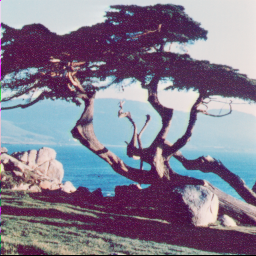
\includegraphics[width=0.8\textwidth]{tree/tree.png}
			\caption{Original}
		\end{subfigure}
		\begin{subfigure}{0.4\textwidth}
			\centering
			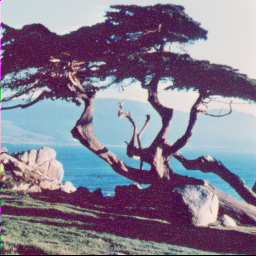
\includegraphics[width=0.8\textwidth]{tree/treetiffBilateralFilter.png}
			\caption{Bilateral}
		\end{subfigure}

		\begin{subfigure}{0.4\textwidth}
			\centering
			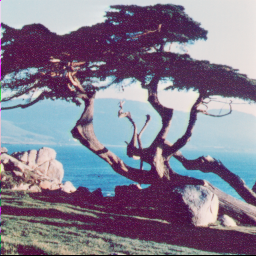
\includegraphics[width=0.8\textwidth]{tree/treetiffGuidedFilter.png}
			\caption{GuidedFilter}
		\end{subfigure}
		\begin{subfigure}{0.4\textwidth}
			\centering
			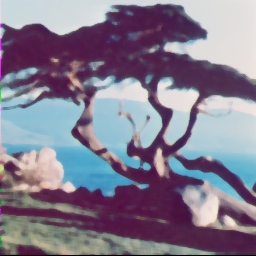
\includegraphics[width=0.8\textwidth]{tree/treetiffMedianFilter.png}
			\caption{Median}
		\end{subfigure}
	
		\begin{subfigure}{0.4\textwidth}
			\centering
			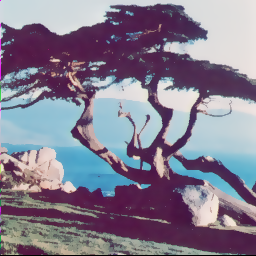
\includegraphics[width=0.8\textwidth]{tree/treetiffRollingGuidanceFilter.png}
			\caption{RollingGuidance}
		\end{subfigure}
		\caption{Landscape image}
	\end{figure}

	\begin{figure}
		\centering
		\begin{subfigure}{0.4\textwidth}
			\centering
			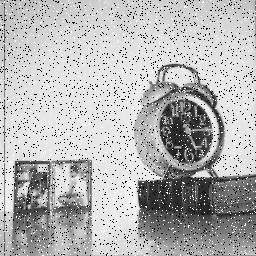
\includegraphics[width=0.8\textwidth]{saltandpepper/SaltAndPepper.png}
			\caption{Original}
		\end{subfigure}
		\begin{subfigure}{0.4\textwidth}
			\centering
			\includegraphics[width=0.8\textwidth]{saltandpepper/SaltAndPepperpngBilateralFilter.png}
			\caption{Bilateral}
		\end{subfigure}
		
		\begin{subfigure}{0.4\textwidth}
			\centering
			\includegraphics[width=0.8\textwidth]{saltandpepper/SaltAndPepperpngGuidedFilter.png}
			\caption{GuidedFilter}
		\end{subfigure}
		\begin{subfigure}{0.4\textwidth}
			\centering
			\includegraphics[width=0.8\textwidth]{saltandpepper/SaltAndPepperpngMedianFilter.png}
			\caption{Median}
		\end{subfigure}
		
		\begin{subfigure}{0.4\textwidth}
			\centering
			\includegraphics[width=0.8\textwidth]{saltandpepper/SaltAndPepperpngRollingGuidanceFilter.png}
			\caption{RollingGuidance}
		\end{subfigure}
		\caption{Salt and pepper noise image}
	\end{figure}

	\begin{figure}
		\centering
		\begin{subfigure}{0.4\textwidth}
			\centering
			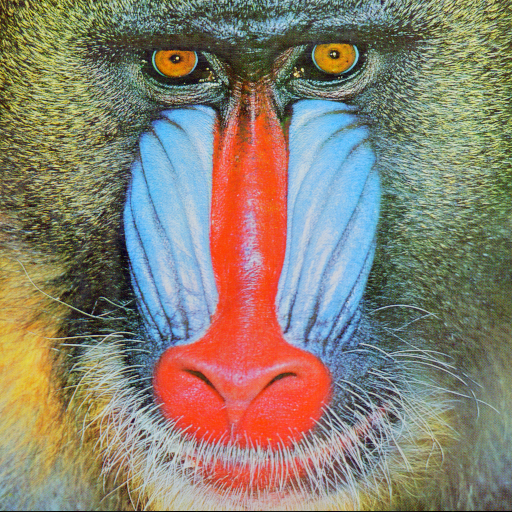
\includegraphics[width=0.8\textwidth]{mandrill/mandrill.png}
			\caption{Original}
		\end{subfigure}
		\begin{subfigure}{0.4\textwidth}
			\centering
			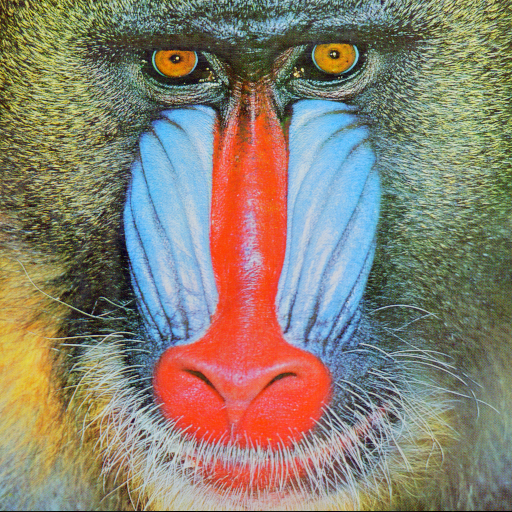
\includegraphics[width=0.8\textwidth]{mandrill/mandrilltiffBilateralFilter.png}
			\caption{Bilateral}
		\end{subfigure}
		
		\begin{subfigure}{0.4\textwidth}
			\centering
			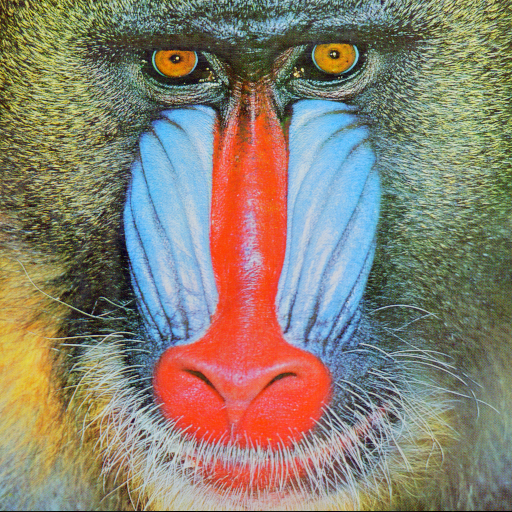
\includegraphics[width=0.8\textwidth]{mandrill/mandrilltiffGuidedFilter.png}
			\caption{GuidedFilter}
		\end{subfigure}
		\begin{subfigure}{0.4\textwidth}
			\centering
			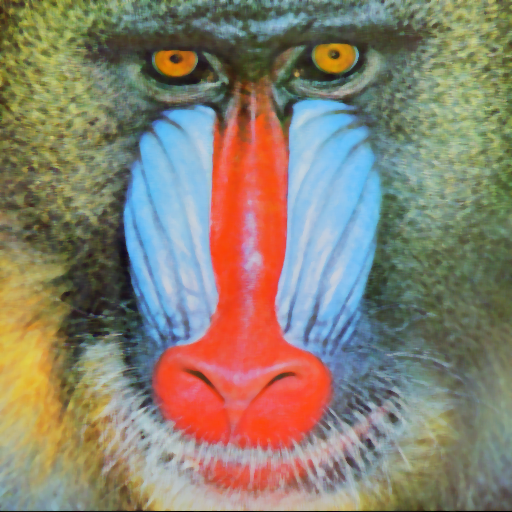
\includegraphics[width=0.8\textwidth]{mandrill/mandrilltiffMedianFilter.png}
			\caption{Median}
		\end{subfigure}
		
		\begin{subfigure}{0.4\textwidth}
			\centering
			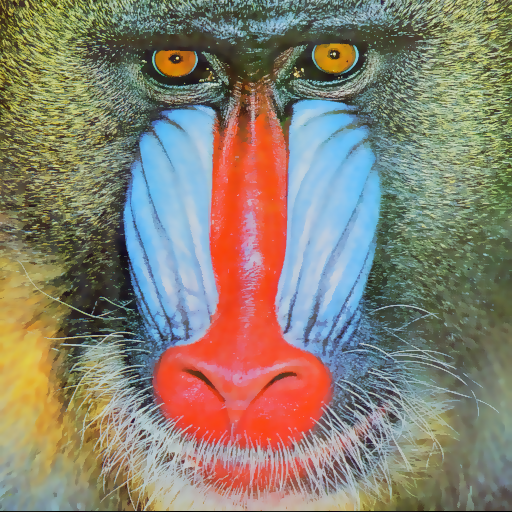
\includegraphics[width=0.8\textwidth]{mandrill/mandrilltiffRollingGuidanceFilter.png}
			\caption{RollingGuidance}
		\end{subfigure}
		\caption{Animal}
	\end{figure}
	
	\begin{figure}
		\centering
		\begin{subfigure}{0.4\textwidth}
			\centering
			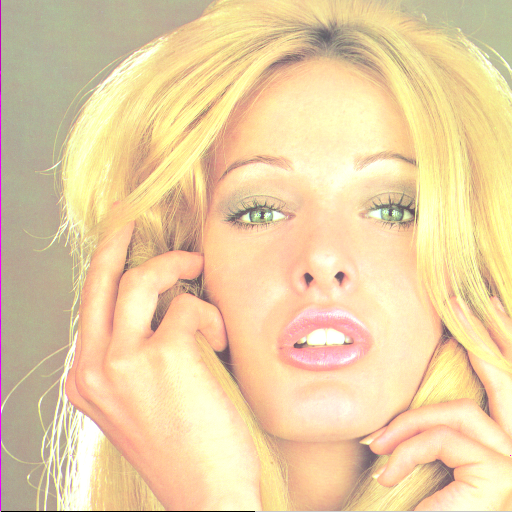
\includegraphics[width=0.8\textwidth]{tiffany/tiffany.png}
			\caption{Original}
		\end{subfigure}
		\begin{subfigure}{0.4\textwidth}
			\centering
			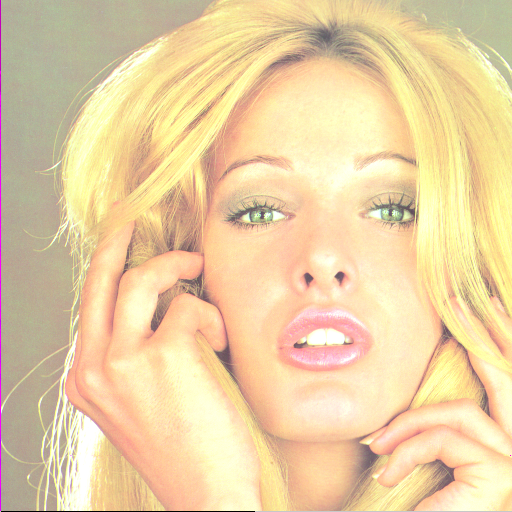
\includegraphics[width=0.8\textwidth]{tiffany/tiffanytiffBilateralFilter.png}
			\caption{Bilateral}
		\end{subfigure}
		
		\begin{subfigure}{0.4\textwidth}
			\centering
			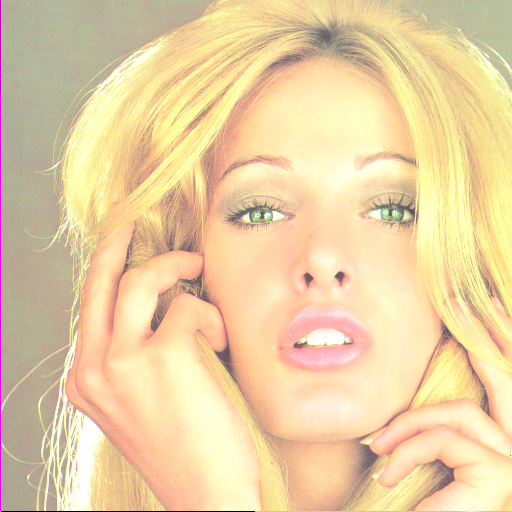
\includegraphics[width=0.8\textwidth]{tiffany/tiffanytiffGuidedFilter.png}
			\caption{GuidedFilter}
		\end{subfigure}
		\begin{subfigure}{0.4\textwidth}
			\centering
			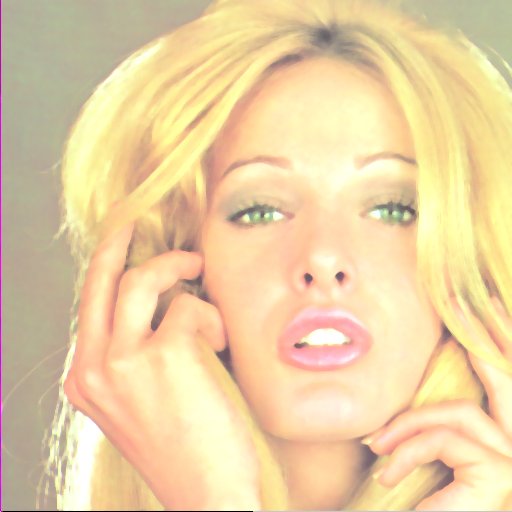
\includegraphics[width=0.8\textwidth]{tiffany/tiffanytiffMedianFilter.png}
			\caption{Median}
		\end{subfigure}
		
		\begin{subfigure}{0.4\textwidth}
			\centering
			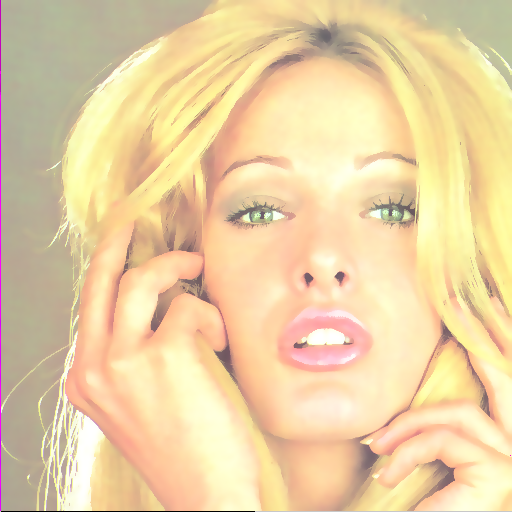
\includegraphics[width=0.8\textwidth]{tiffany/tiffanytiffRollingGuidanceFilter.png}
			\caption{RollingGuidance}
		\end{subfigure}
		\caption{Portrait}
	\end{figure}

	\begin{figure}
		\centering
		\begin{subfigure}{0.4\textwidth}
			\centering
			
\includegraphics[width=0.8\textwidth]{document/document.jpg}
			\caption{Original}
		\end{subfigure}
		\begin{subfigure}{0.4\textwidth}
			\centering
			
\includegraphics[width=0.8\textwidth]{document/documentjpgBilateralFilter.png}
			\caption{Bilateral}
		\end{subfigure}
		
		\begin{subfigure}{0.4\textwidth}
			\centering
			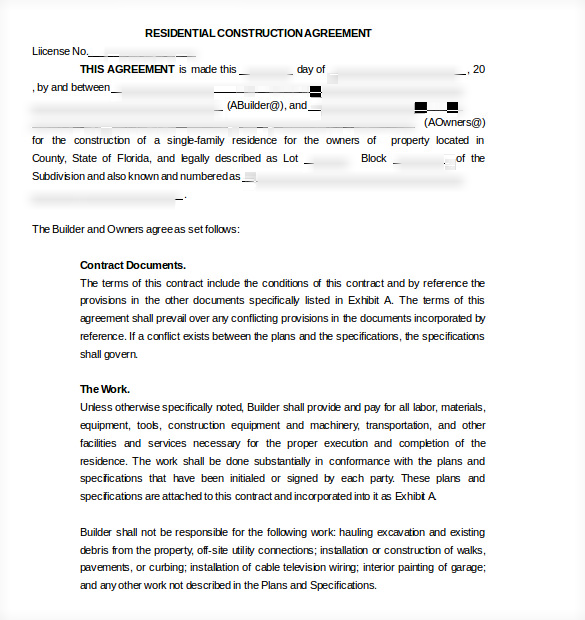
\includegraphics[width=0.8\textwidth]{document/documentjpgGuidedFilter.png}
			\caption{GuidedFilter}
		\end{subfigure}
		\begin{subfigure}{0.4\textwidth}
			\centering
			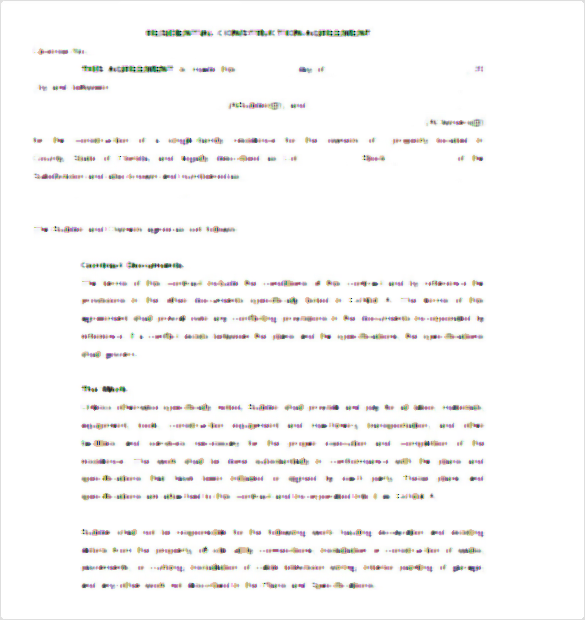
\includegraphics[width=0.8\textwidth]{document/documentjpgMedianFilter.png}
			\caption{Median}
		\end{subfigure}
		
		\begin{subfigure}{0.4\textwidth}
			\centering
			
\includegraphics[width=0.8\textwidth]{document/documentjpgRollingGuidanceFilter.png}
			\caption{RollingGuidance}
		\end{subfigure}
		\caption{Document}
	\end{figure}
\end{document}
